\textbf{Цель работы:} исследовать энергетическую зависимость вероятности рассеяния электронов атомами ксенона, 
определить энергии электронов, при которых наблюдается <<просветление>> ксенона, и оценить размер его внешней электронной оболочки, 
глубину потенциальной ямы и потенциал ионизации.

\textbf{Используемое оборудование:} тиратрон ТГ3-01/1.3Б, осциллограф, стабилизированный блок накала электрода.  

\section{Теоретическое введение}

	В результате исследований зависимости поперечных сечений упругого рассеяния электронов (с энергией до 10 ЭВ) 
	на атомах аргона было обнаружено явление, получившее название \textit{эффекта Рамзауэра}.
		
	С точки зрения квантовой теории атом по отношению к электронной волне ведет себя 
	как преломляющая среда с относительным показателем преломления
		\begin{equation}
			n = \frac{\lambda}{\lambda^\prime} = \sqrt{1-\frac{U}{E}},
		\end{equation}
	где $U$, $E$ -- соответственно потенциальная и полная энергии электрона внутри атома.
		
	Будем считать, что электрон рассеивается на одномерной прямоугольной потенциальной яме конечной глубины. 
	Такая модель является хорошим приближением для атомов тяжелых инертных газов, отличающихся наиболее компактной структурой и резкой внешней границей. 
	Решение задачи о прохождении частицы с энергией $E$ над потенциальной ямой шириной $l$ и глубиной $U_0$ не составит труда найти из уравнения Шредингера:\\
		\begin{equation}
			\psi^{\prime\prime}+k^2\psi=0, \ \text{где}\
			k^2 =\begin{cases}
				2mE/\hbar^2 & x<0, x>l\\
				2m(E+U_0)/\hbar^2 & 0<x<l
			\end{cases}.
		\end{equation}

	Коэффициент прохождения равен отношению квадратов амплитуд прошедшей и падающей волн и определяется выражением:
		\begin{equation}
			\frac{1}{D} = 1 + \frac{U_0^2}{4E(E+U_0)}\sin^2(k_2l).
		\end{equation}

	Минимум последнего выражения отвечает квантовому аналогу просветления оптики, так как при выполнении условия
	\begin{equation}
		\label{coeff_minimal}
		\sqrt{\frac{2m(E+U_0)}{\hbar^2}}l = \pi n, \ n\in\mathbb{N},
	\end{equation}
	коэффициент прохождения частицы над ямой становится равным единице, то есть достигает своего максимального значения.

	Отметим, что условие \eqref{coeff_minimal} легко получить, рассматривая интерференцию электронов волн де Бройля в атоме:\\
	Условие первого интерференционного максимума:
	\begin{equation}
		\label{eq:1}
		2l = \frac{h}{\sqrt{2m(E_1+U_0)}}.
	\end{equation}

	Условие первого интерференционного минимума:
	\begin{equation}
		\label{eq:2}
		2l =\frac{3}{2} \frac{h}{\sqrt{2m(E_2+U_0)}}.
	\end{equation}			

	Решая совместно уравнения~(\ref{eq:1}, \ref{eq:2}) можно получить:
	\begin{equation}
		\label{eq:3}
		l = \frac{h\sqrt{5}}{\sqrt{32m(E_2-E_1)}}.
	\end{equation}
	Понятно, что энергии $E_1$ и $E_2$ соответствуют энергиям электронов, прошедших разность потенциалов $V_1$ и $V_2$, то есть $E_1 = eV_1$ и $E_2 = eV_2$. 
	
	По измеренным величинам $E_1$ и $E_2$, используя формулы~(\ref{eq:1}, \ref{eq:2}), можно рассчитать эффективную глубину потенциальной ямы атома:
	\begin{equation}
		\label{eq:U_0}
		U_0 = \frac{4}{5}E_2 - \frac{9}{5}E_1
	\end{equation}

\section{Экспериментальная установка}

	В нашей работе для изучения эффекта Рамзауэра используется тиратрон ТГ3-01/1.3Б, заполненный инертным газом. 
	Принципиальная схема установки для изучения эффекта Рамзауэра и схематическое изображение тиратрона и его конструкция приведены на рис.~\ref{setup1}.
		
	На лампу Л подаётся синусоидальное напряжение частоты 50 Гц от источника питания ИП, 
	С -- стабилизированный блок накала катода; исследуемый сигнал подаётся на электронный осциллограф (ЭО); цифрами обозначены номера ножек лампы.
		
	\begin{figure}[h!]
		\begin{center}
			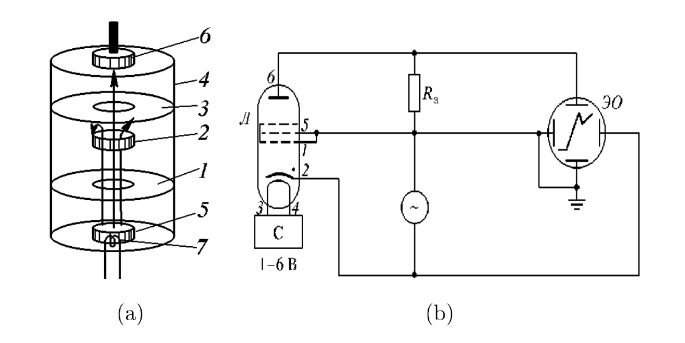
\includegraphics[width = 14 cm]{images/setup}
			\caption{Схема экспериментальной установки}
			\label{setup1}
		\end{center}
	\end{figure}

	Лампа-тиратрон ТГ3-01/1.3Б, заполненная инертным газом, расположена непосредственно на корпусе блока источника питания (БИП). 
	Напряжение к электродам лампы подаётся от источников питания, находящихся в корпусе прибора. 
	Регулировка напряжения и выбор режима работы установки производится при помощи ручек управления, выведенных на лицевую панель БИП.
		
	Зависимость вероятности рассеяния электрона от его энергии можно определить, зная ВАХ тиратрона:
	\begin{equation}
		\label{eq:w}
		w(U) = -\frac{1}{C}\ln \frac{I_a(U)}{I_0},
	\end{equation}
	где $I_0$ -- ток катода, а $C$ -- некторая постоянная.
	
\section{Ход работы}


\subsection*{Динамический режим работы}

\begin{enumerate}
    
    \item Включим динамический режим и установим напряжение накала лампы равное $(3.11 \pm 0.01) \text{ В}$.
    \item Подкручивая ручкой фазу, сведём прямой и обратной ход характерестик. 
    \item Измерим напряжение между сеткой и катодом, которое соответствует максимуму, минимуму харастеристик и пробою тиратрона. Ноль напряжения определяем при заземлении входа.
    \item Повторим измерения для напряжение накала лампы $(2.81 \pm 0.01) \text{ В}$.

	\begin{figure}[H]
		\centering
		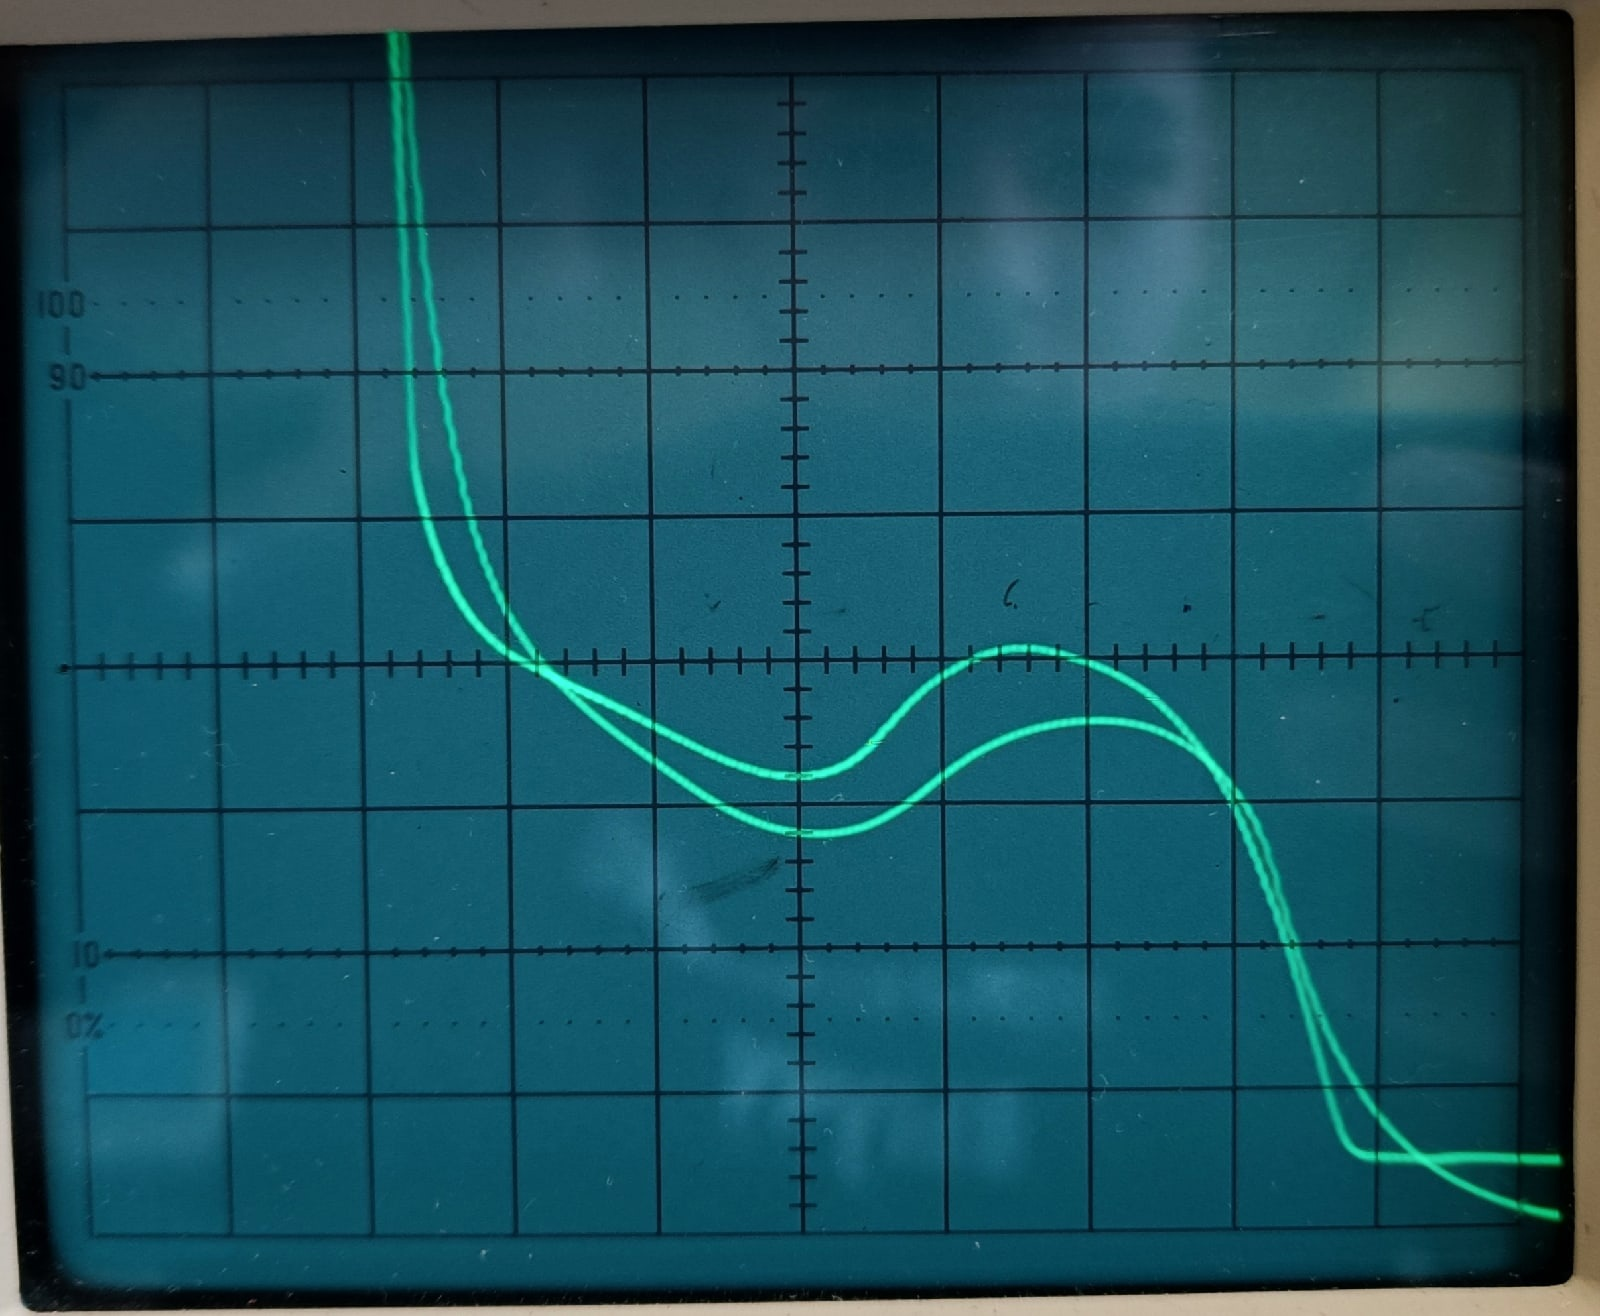
\includegraphics[width = 11 cm]{images/osc_311}
		\caption{$U_{\text{нак}} = (3.11 \pm 0.01) \text{ В}$}
		\label{VAH_311}
	\end{figure}

	\begin{figure}[H]
		\centering
		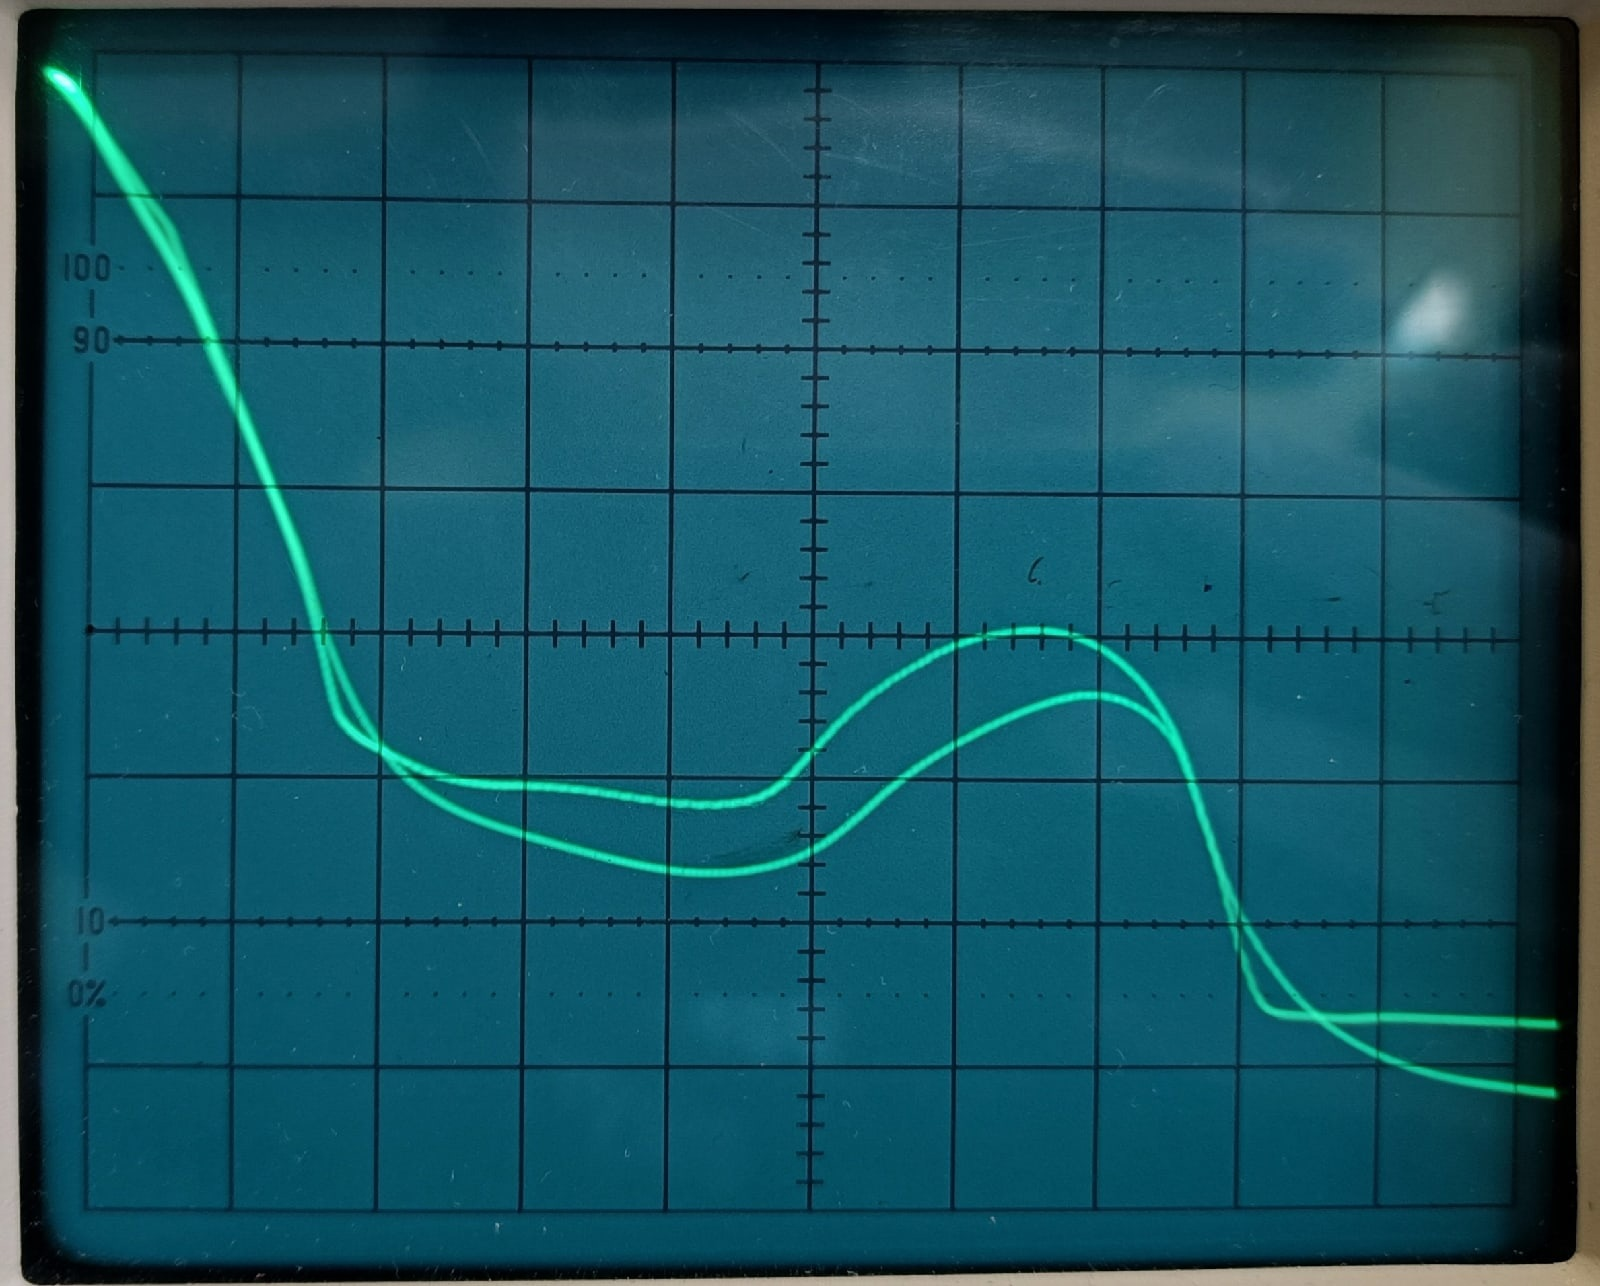
\includegraphics[width = 11 cm]{images/osc_281}
		\caption{$U_{\text{нак}} = (2.81 \pm 0.01) \text{ В}$}
		\label{VAH_281}
	\end{figure}

    \begin{table}[h!]
        \centering
        \begin{tabular}{|c|c|c|c|}
        \hline
        $U_{\text{нак}}$, В & $V_{max}$, В & $V_{min}$, В & $V_{\text{пробоя}}$, В \\ \hline
        $3.11 \pm 0.01$ & $6.0 \pm 0.4$ & $10.0 \pm 0.4$ & $14.4 \pm 0.4$    \\ \hline
        $2.81 \pm 0.01$ & $4.6 \pm 0.4$ & $10.0 \pm 0.4$ & $14.4 \pm 0.4$    \\ \hline
        \end{tabular}
        \caption{Результаты измерений в динамическом режиме}
    \end{table}

    % \item Поднесём постоянный магнит к лампе. ВАХ тиратрон можно полностью погасить путём добавления магнитного поля, электроны, испытавшие упругое столкновение, отклоняются ещё сильнее. 
    \item По результатам измерений в динамическом режиме рассчитаем размер электронной оболочки атома инертного газа, заполняющего лампу, 
    приняв $U_0 = 2,5 \text{ В}$, по формулам $\eqref{eq:1}$ и $\eqref{eq:2}$. Исключив $U_0$, рассчитаем размер электронной оболочки атома этого газа по формуле $\eqref{eq:3}$.

    \[ l_1 = \frac{h}{2\sqrt{2m(E_1+U_0)}}, ~\sigma_{l_1} = l_1 \frac{\sigma_{E_1}}{2(E_1 + U_0)}\]
    \[ l_2 = \frac{3h}{4\sqrt{2m(E_2+U_0)}}, ~\sigma_{l_2} = l_2 \frac{\sigma_{E_2}}{2(E_2 + U_0)}\]
    \[ l_3 = \frac{h\sqrt{5}}{\sqrt{32m(E_2-E_1)}}, ~\sigma_{l_3} = l_3 \frac{\sigma_{E_2} + \sigma_{E_1}}{2(E_2 - E_1)}\]

    \item Оценим глубину потенциальной ямы по формуле $\eqref{eq:U_0}$. Видим, что полученные результаты отличаются от предложенной модели. 
    \item По результатам напряжения пробоя, оценим ионизации инертного газа, как $U_{проб} +  U_0$. Наиболее близкое значение у ксенона -- $12.1 \text{ эВ}$.
    \begin{table}[h!]
        \centering
        \begin{tabular}{|c|c|c|c|c|c|}
        \hline
        $U_{\text{нак}}$, В & $l_1$, \AA      & $l_2$, \AA      & $l_3$, \AA      & $U_0$, эВ & $U_{ион}$,  эВ \\ \hline
        $3.11 \pm 0.01$    & $2,10 \pm 0,05$ & $2,59 \pm 0,04$ & $3,42 \pm 0,34$ & $ -2.8 \pm 1.0 $ & $11.6 \pm 1.4$ \\ \hline
        $2.81 \pm 0.01$    & $2,30 \pm 0,07$ & $2,59 \pm 0.04$ & $2.94 \pm 0,22$ & $ -0.3 \pm 1.0 $  & $14.1 \pm 1.4$ \\ \hline
        \end{tabular}
        \caption{Результаты динамического способа}
    \end{table}
     
\end{enumerate}

\subsection*{Статический режим работы}

	\begin{enumerate}
		\item Перейдем к измерению ВАХа в статическом режиме. 
		Ток на аноде определяется по показанию вольтметра $(V_{\text{анод}})$, делённому на сопротивление $100 \text{ кОм}$, которое включено в цепь анода. 
		$\sigma_{V_{\text{анод}}} = 0.01 \text{ мВ}$.
		\item Построим графики $I_{\text{анод}} = f(V_{\text{катод}})$.

		\begin{figure}[H]
			\centering
			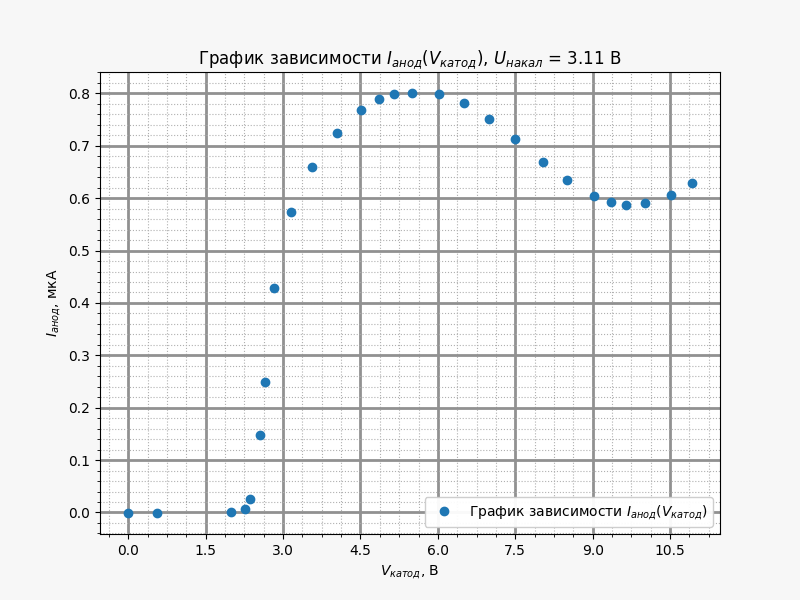
\includegraphics[width = 12 cm]{images/U_311}
			\caption{$U_{\text{нак}} = (3.11 \pm 0.01) \text{ В}$}
			\label{U311}
		\end{figure}

		\begin{figure}[H]
			\centering
			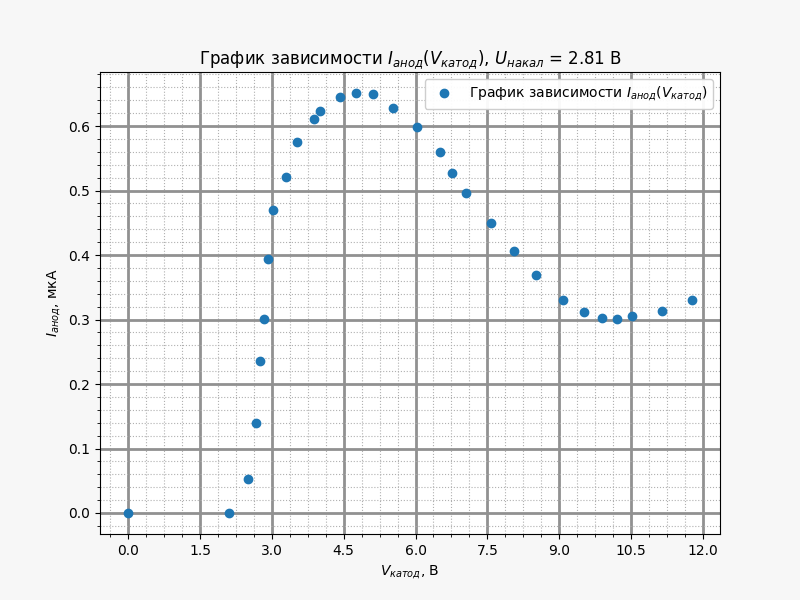
\includegraphics[width = 12 cm]{images/U_281}
			\caption{$U_{\text{нак}} = (2.81 \pm 0.01) \text{ В}$}
			\label{U281}
		\end{figure}
	
		\item По значениям графиков оценим следующие значения:
		\begin{table}[h!]
			\centering
			\begin{tabular}{|c|c|c|}
			\hline
			$U_{\text{нак}}$, В & $V_{max}$, В & $V_{min}$, В   \\ \hline
			$3.11 \pm 0.01$ & $5.5 \pm 0.3$ & $9.7 \pm 0.3$     \\ \hline
			$2.81 \pm 0.01$ & $4.7 \pm 0.3$ & $10.2 \pm 0.3$    \\ \hline
			\end{tabular}
			\caption{Результаты измерений в статическом режиме}
		\end{table}
		\item Вычисляем те же величины, что и динамическом режиме. 
		\begin{table}[h!]
			\centering
			\begin{tabular}{|c|c|c|c|c|c|}
			\hline
			$U_{\text{нак}}$, В & $l_1$, \AA      & $l_2$, \AA      & $l_3$, \AA      & $U_0$, эВ  \\ \hline
			$3.11 \pm 0.01$    & $2,16 \pm 0,04$ & $2,62 \pm 0,03$ & $3,34 \pm 0,24$ & $ -2.1 \pm 0.8 $ \\ \hline
			$2.81 \pm 0.01$    & $2,28 \pm 0,05$ & $2,57 \pm 0.03$ & $2.92 \pm 0,16$ & $ -0.3 \pm 0.8 $  \\ \hline
			\end{tabular}
			\caption{Результаты статического режима}
		\end{table}

		\item Оценим при каких напряжениях должны появляться максимумы в коэффециенте прохождения электронов для $n = 2, 3$
		\[ k_2 l = \sqrt{\frac{2m (E_n + U_0)}{\hbar^2}} l = n \pi ~\Rightarrow~ E_n = - U_0 + \frac{h^2 n^2}{8m l^2}\]

		Для оценки возьмём, как $U_0 = - 1.4 \text{ эВ}$ и $l = 2,65$ \AA -- средние измеренные значения. 
		\[ E_n = 1.4 + 5.3 \cdot n^2 \text{ эВ}~\Rightarrow~ E_2 = 22,6 \text{ эВ}, ~E_3 = 49,1 \text{ эВ} \]

		Следующие максимумы выше потенциала ионизации, поэтому мы не можем их наблюдать.

		\item Найдём токи $I_0$ из предыдущих графиков - они соответствуют найденным максимумам. $I_0 = (803 \pm 2) \text{ пА}$ при $U_{\text{нак}} = (3.11 \pm 0.01) \text{ В}$. 
		$I_0 = (652 \pm 3) \text{ пА}$ при $U_{\text{нак}} = (2.81 \pm 0.01) \text{ В}$.
		
		Найдём зависимость вероятности рассеяния электронов от энергии c коэффициентом в виде константы $C$:

		\begin{figure}[H]
			\centering
			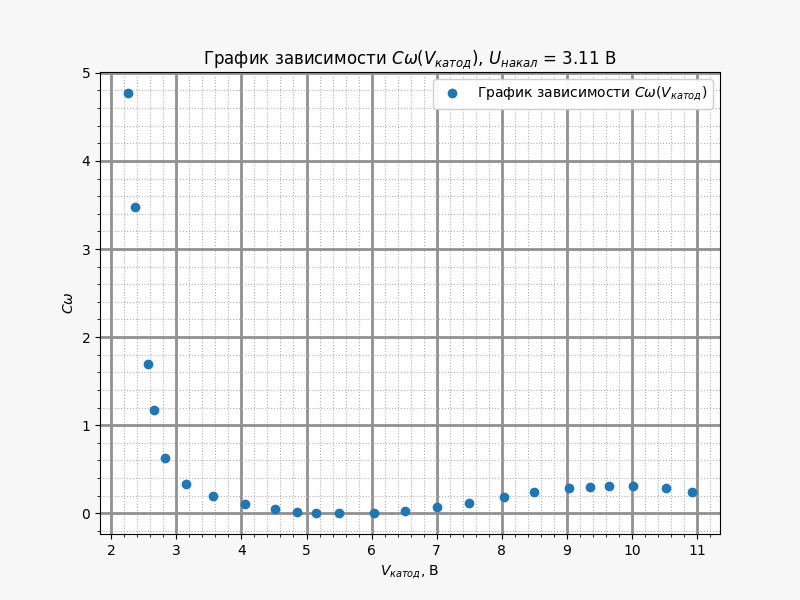
\includegraphics[width = 12 cm]{images/probability_311}
			\caption{$U_{\text{нак}} = (3.11 \pm 0.01) \text{ В}$}
			\label{prob_311}
		\end{figure}

		\begin{figure}[H]
			\centering
			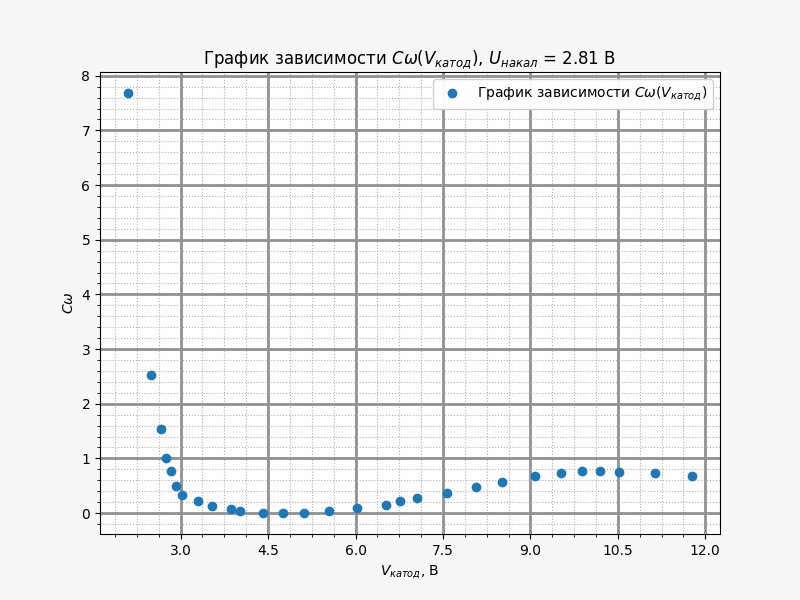
\includegraphics[width = 12 cm]{images/probability_281}
			\caption{$U_{\text{нак}} = (2.81 \pm 0.01) \text{ В}$}
			\label{prob_281}
		\end{figure}
		
	\end{enumerate}

	

\section{Заключение}

	В ходе работы был изучен ВАХ тиратрона в динамическом и статическом режимах при различных напряжениях накала. 
    С помощью измерений ВАХа тиратрона удалось установить, какой инертный газ использовался в работе: 
    по напряжению пробоя была получена энергия ионизация газа, которая оказалась примерно равна энергии ионизации ксенона -- $12.1 \text{ эВ}$. 

    Также удалось оценить размер электронной оболочки разными метода, в среднем полученный результат $l = (2.65 \pm 0.30)$ \AA, что соответствует значению для ксенона $l = 2.80$ \AA. 
    А также глубину потенциальной ямы $U_0 = (- 1.4 \pm 0.8) \text{ эВ}$. Полученное значение показывает, что для подсчёта истинного значения требуется применения другой модели.

    \begin{table}[h!]
        \centering
        \begin{tabular}{|c|c|c|c|c|c|}
        \hline
        $U_{\text{нак}}$, В & $l_1$, \AA      & $l_2$, \AA      & $l_3$, \AA      & $U_0$, эВ & $U_{ион}$,  эВ \\ \hline
        $3.11 \pm 0.01$    & $2,10 \pm 0,05$ & $2,59 \pm 0,04$ & $3,42 \pm 0,34$ & $ -2.8 \pm 1.0 $ & $11.6 \pm 1.4$ \\ \hline
        $2.81 \pm 0.01$    & $2,30 \pm 0,07$ & $2,59 \pm 0.04$ & $2.94 \pm 0,22$ & $ -0.3 \pm 1.0 $  & $14.1 \pm 1.4$ \\ \hline
        \end{tabular}
        \caption{Результаты динамического способа}
    \end{table}

    \begin{table}[h!]
        \centering
        \begin{tabular}{|c|c|c|c|c|c|}
        \hline
        $U_{\text{нак}}$, В & $l_1$, \AA      & $l_2$, \AA      & $l_3$, \AA      & $U_0$, эВ  \\ \hline
        $3.11 \pm 0.01$    & $2,16 \pm 0,04$ & $2,62 \pm 0,03$ & $3,34 \pm 0,24$ & $ -2.1 \pm 0.8 $ \\ \hline
        $2.81 \pm 0.01$    & $2,28 \pm 0,05$ & $2,57 \pm 0.03$ & $2.92 \pm 0,16$ & $ -0.3 \pm 0.8 $  \\ \hline
        \end{tabular}
        \caption{Результаты статического режима}
    \end{table}

